\chapter{Target tracking}
Target tracking plays a pivotal role in radar systems, where the primary objective is to estimate the trajectory and characteristics of moving objects within a surveillance area. Derived from the foundational principles of the Kalman filter, target tracking algorithms are tailored to the specific requirements and challenges inherent in radar applications.

Radar-based target tracking encounters various complexities, including survivability and the presence of crossing targets. Survivability concerns the algorithm's ability to maintain accurate estimates despite target maneuvers, occlusions, or potential target loss. Furthermore, the phenomenon of crossing targets introduces significant ambiguities and challenges in trajectory estimation and association.

In the realm of single-target tracking, algorithms such as the Probabilistic Data Association (PDA) filter and its derivatives, such as the Joint Probabilistic Data Association (JPDA) filter or the Integrated Probabilistic Data Association (IPDA) filter, are commonly employed. These algorithms provide robust solutions for associating measurements with existing tracks and updating target state estimates in dynamic scenarios.

Beyond single-target tracking, radar systems often necessitate multi-target tracking approaches. These approaches, particularly those based on Random Finite Sets (RFS), offer advanced capabilities for tracking multiple targets simultaneously. RFS-based filters, including the Probability Hypothesis Density (PHD) filter and the Multi-Bernoulli filter, excel in scenarios where the number of targets is uncertain or dynamic.

In this chapter, we delve into the intricacies of radar-based target tracking algorithms, exploring their theoretical foundations, practical implementations, and performance characteristics. By understanding the diverse range of tracking algorithms available and their respective strengths, we can design and deploy effective tracking systems to meet the demands of modern surveillance and reconnaissance applications.

\section{Data association}
\label{sec:data_association}
Data association uncertainty arises in remote sensing systems, such as radar, sonar, or electro-optical devices, when
measurements are obtained from sources that may not necessarily be the target of interest \cite{BarShalomPDA}. This uncertainty
occurs particularly in situations where the target signal is weak, necessitating a lower detection threshold, which may result in the detection of background signals, sensor noise, or clutter. Additionally, data association uncertainty can occur when multiple targets are present in close proximity. Utilizing spurious measurements in a tracking filter can lead to divergence of the estimation error and, consequently, track loss.

Addressing this challenge involves two primary problems. The first is the selection of appropriate measurements to update the state of the target of interest in the tracking filter, which can be a Kalman filter or an extended Kalman filter (EKF). The second problem involves determining whether the filter needs modification to account for data association uncertainty. The objective is to obtain the minimum mean square error (MMSE) estimate of the target state and associated uncertainty.

The optimal estimator involves the recursive computation of the conditional probability density function (pdf) of the
state, with detailed conditions provided under which this pdf serves as a sufficient statistic in the presence of
data association uncertainty.
  \subsection{Validation region}
    \label{sec:validation_region}
In target-tracking scenarios, the process of signal detection provides measurements, from which the appropriate ones for inclusion in the target state estimator are chosen. In radar systems, for instance, the signal reflected from the target of interest is sought within a specific time interval, determined by the expected range of the target when it reflects the transmitted energy. A range gate is established, and detections falling within this gate can be associated with the target of interest. These measurements may include parameters such as range, azimuth, elevation, or direction cosines, and in certain cases, range rate for radar or active sonar; bearing, and potentially frequency, time difference of arrival, and frequency difference for passive sonar; as well as line-of-sight angles or direction cosines for optical sensors. By setting up a multidimensional gate, the signal from the target is detected efficiently, avoiding the need to search for it across the entire measurement space.

However, while a measurement within the gate is a candidate for association with the target, it is not guaranteed to have originated from the target itself. Thus, the establishment of a validation region becomes necessary. The validation region is designed to ensure that the target measurement falls within it with a high probability, known as the gate probability, based on the statistical characterization of the predicted measurement. In the event that more than one detection appears within the gate, association uncertainty arises. This uncertainty entails the need to determine which measurement is truly from the target and should therefore be utilized to update the track, which comprises the state estimate and covariance, or more generally, the sufficient statistic for the target in question. Measurements outside the validation region can be disregarded, as they are too distant from the predicted measurement and are unlikely to have originated from the target of interest. This scenario typically arises when the gate probability is close to unity, and the statistical model used to define the gate is accurate.
\section{Clutter}
When it comes to clutter, two scenarios may occur. The first one is a single target in a clutter. This problem of
tracking a single target in a clutter appears when several measurements appear in the validation region. The
validated measurements comprise the accurate measurement, if detected within this region, along with spurious
measurements originating from clutter or false alarms. In air traffic control systems, where cooperative targets are
involved, each measurement includes a target identifier known as the squawk number. If this identifier is entirely
reliable, data association uncertainty is eliminated. However, in cases where a potentially hostile target is non
-cooperative, data association uncertainty becomes a significant challenge.

Figure \ref{fig:singleTargetInClutter} illustrates a scenario involving multiple validated measurements. The validation region depicted in the
figure is two-dimensional and takes the form of an ellipse centered at the predicted measurement $\hat{z}$. The
elliptical shape of the validation region arises from the assumption that the error in the target's predicted
measurement, known as the innovation, follows a Gaussian distribution. The parameters defining the ellipse are
determined by the covariance matrix $S$ of the innovation.

All measurements within the validation region have the potential to originate from the target of interest, although
only one of them is the true measurement. As a result, the possible association events include: $z_1$ originating
from the target, with $z_2$ and $z_3$ being from clutter; $z_2$ originating from the target, with $z_1$ and $z_3$
being from clutter; $z_3$ originating from the target, with $z_2$ and $z_1$ being from clutter; or all measurements
being from clutter. These association events are mutually exclusive and exhaustive, enabling the application of the
total probability theorem to obtain the state estimate in the presence of data association uncertainty.

Under the assumption of a single target, the spurious measurements are considered random interference. A common model for such false measurements assumes that they are uniformly spatially distributed and independent across time, corresponding to residual clutter. Any constant clutter is assumed to have already been removed.

\begin{figure}[h]
  \centering
  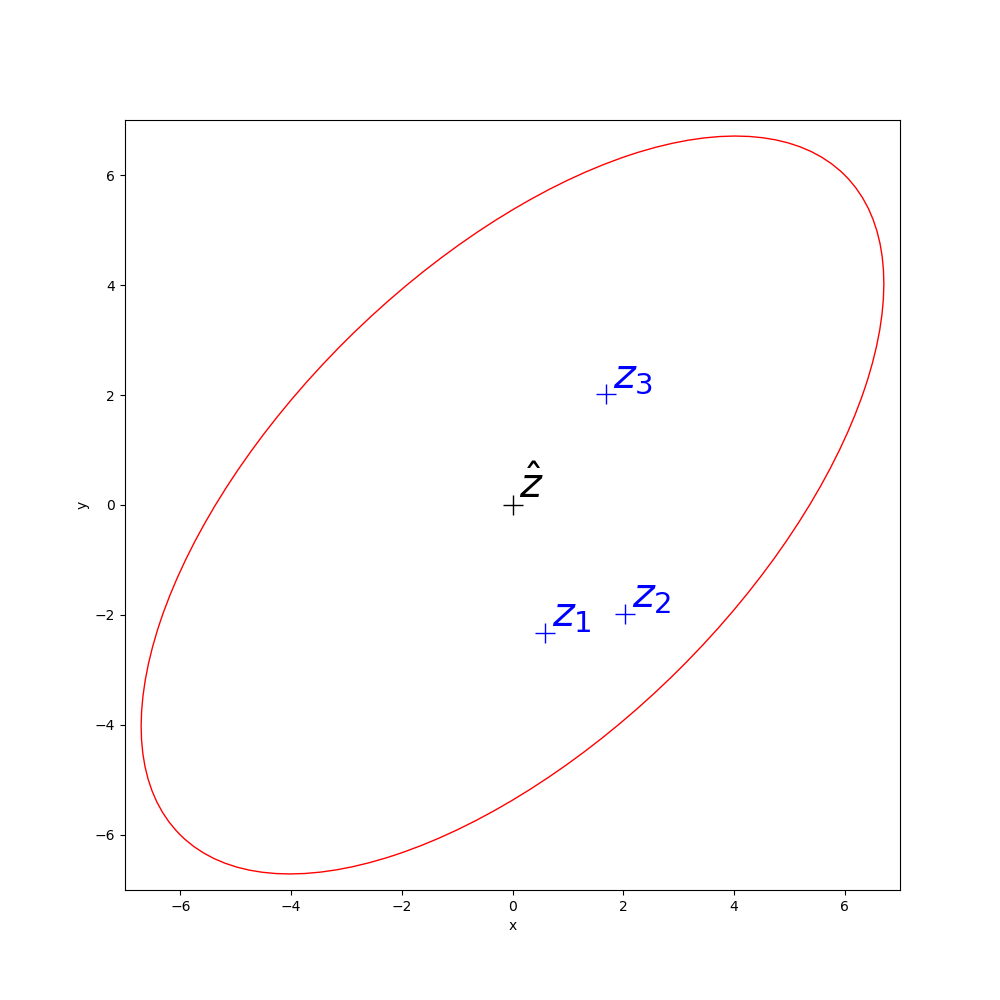
\includegraphics[width=10cm]{text/chapter_02/imgs/clutter_singleTarget}
  \caption{Several measurements $z_i$ appeared in the validation region of a single target. $\hat{z}$ is a predicted
  measurement and none or any of the measurement $z_1 - z_3$ may have originated from the target.}
  \label{fig:singleTargetInClutter}
\end{figure}

When several targets as well as a clutter or false alarms appear in the same neighbour, the data association becomes even more challenging. Figure \ref{fig:twoTargetsInClutter} shows this scenario, where predicted measurement for the targets are close to each other. These predicted points are labeled as $\hat{z_1}$ and $\hat{z_2}$. In This Figure many association combinations are possible; $z_1$ from target $\hat{z_1}$ or clutter; $z_2$ from target $\hat{z_1}$ or clutter; $z_4$ from target $\hat{z_2}$ or clutter; $z_3$ from target $\hat{z_1}$ or targe $\hat{z_2}$ or clutter. However, if $z_3$ originated from target $\hat{z_1}$, then it probable, that $z_4$ originated from target $\hat{z_2}$.

This scenario demonstrates the intricate relationships among associations when persistent interference from neighboring targets coexists with random interference or clutter. In such cases, joint association events become necessary to properly account for these dependencies.

A more complex scenario may arise due to the inherent finite resolution capability of signal processing systems. While each measurement is typically assumed to originate from either a target or clutter, an additional possibility must be considered: the merging of detections from multiple targets. Specifically, measurement $z_3$ could potentially result from such merging, representing an unresolved measurement. This introduces a fourth origin hypothesis for a measurement lying within the intersection of two validation regions.

The discussion highlights the challenges associated with associating measurements to tracks. The complete problem involves associating measurements at each time instant, updating the track's sufficient statistic, and propagating it to the subsequent time instant.

\begin{figure}[h]
    \centering
    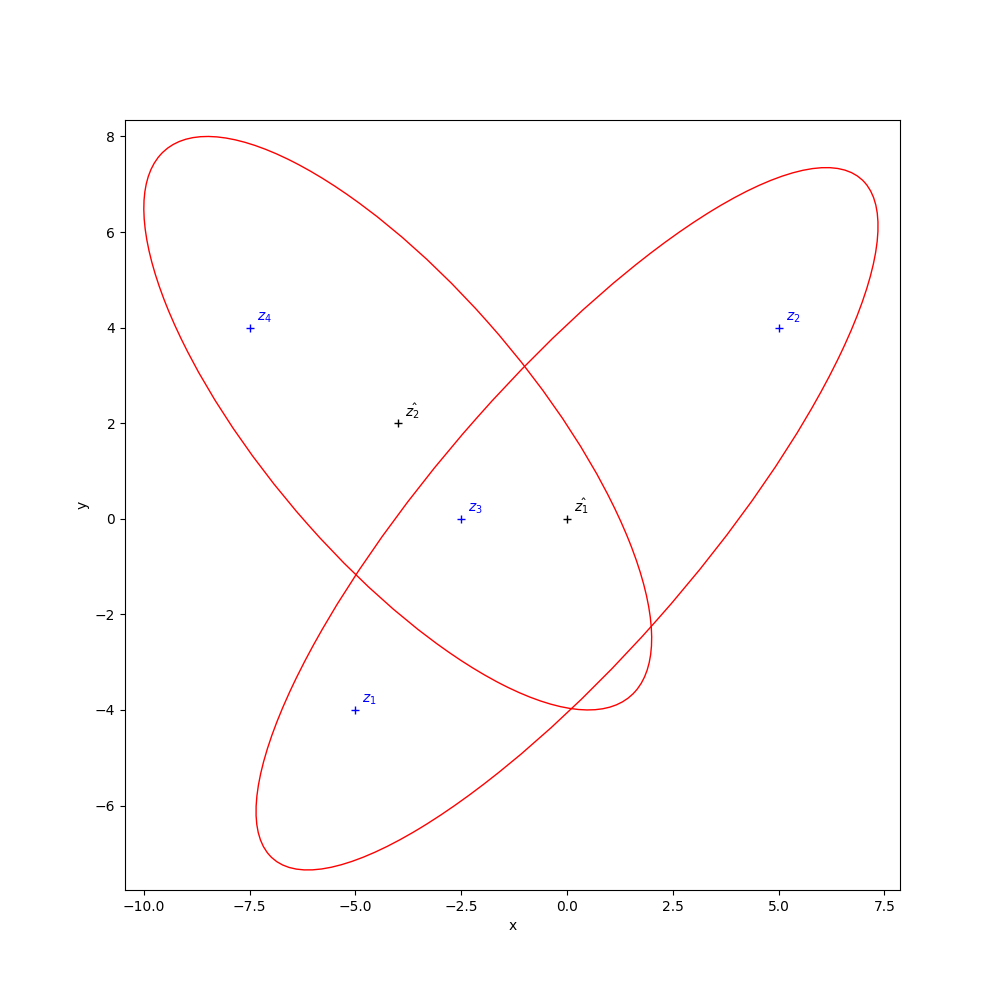
\includegraphics[width=10cm]{text/chapter_02/imgs/clutter_multiTarget}
    \caption{Several measurements $z_i$ appeared in the validation region of one of targets $\hat{z_1}$ or $\hat{z_2}$. $\hat{z_1}$ and $\hat{z_2}$ are predicted
    measurements and none or any of the measurement $z_1 - z_3$ may have originated from the target $\hat{z_1}$ and none or any of the measurement $z_3 - z_4$ may have originated from the target $\hat{z_2}$.}
    \label{fig:twoTargetsInClutter}
\end{figure}


\section{Single target tracking}
Single Target Tracking algorithms are specifically designed to track a single target amidst clutter and other sources of interference. Unlike conventional Kalman filters, which are not inherently equipped to handle clutter, Single Target Tracking algorithms incorporate mechanisms to enhance target survivability in cluttered environments.

One prominent algorithm in the data association category of target tracking is the Probabilistic Data Association (PDA) filter. The PDA filter addresses the challenge of associating measurements with the correct target while accounting for data association uncertainty. This uncertainty arises from the presence of clutter and the possibility of spurious measurements.


\subsection{PDA filter}
\label{sec:pda_filter}
The Probabilistic Data Association (PDA) algorithm computes the association probabilities for each validated measurement at the current time with respect to the target being tracked. This probabilistic or Bayesian information serves as a foundation for the Probabilistic Data Association Filter (PDAF) tracking algorithm, which effectively addresses the uncertainty regarding the origin of measurements. In scenarios where the state and measurement equations are linear, the resulting PDAF algorithm operates based on the Kalman Filter (KF). However, if the state or measurement equations are nonlinear, the PDAF algorithm is instead based on the Extended Kalman Filter (EKF). This adaptation allows the PDAF algorithm to accommodate nonlinearity in the system dynamics or measurement processes, ensuring robust performance in diverse tracking scenarios.

The PDAF algorithm comes with many assumptions:
\begin{enumerate}
    \item Only one target of interest is present, whose state $x \in R^{n_x}$ is assumed to evolve in time according to the equation
        \begin{align}
            x_k &= F_{k-1} x_{k-1} + \mu_{k-1},
        \end{align}
        with the true measurement $z_k \in R^{n_z}$ given by
        \begin{align}
            \label{eq:pda_A1_eq2}
            z_k &= H_k x_k + w_k,
        \end{align}
        where $\mu_{k-1}$ and $w_k$ are zero mean mutually independent, white Gaussian noise variables with covariances $Q_{k-1}$ and $R_k$, respectively.
    \item The track has been initialized.
    \item The past information through time $k-1$ about the target is summarized approximately by a suffifient statistic in the form of the Gaussian posterior
        \begin{align}
            p(x_{k-1}|z_{k-1}) &= \mathcal{N}(x_{k-1}; x_{k-1|k-1}, P_{k-1|k-1})). \label{eq:pda_A3}
        \end{align}
    \item At each time a measurement validation region is set up around the predicted measurement to select the candidate measurements for association to the target of interest.
    \item If the target was detected and the corresponding
    measurement fell into the validation region, then,
    according to (\ref{eq:pda_A1_eq2}), at most one of the validated measurements can be target originated.
    \item The remaining measurements are assumed to be due
    to false alarms or clutter and are modeled as inde-
    pendent and identically distributed with uniform spatial distribution, and the number of false alarms or clutter points obeys either a Poisson distri-
    bution, that is, a spatial Poisson process, with known
    spatial density $\lambda$, or a diffuse prior.
    \item The target detections occur independently over time
    with known probability $p_D$.
\end{enumerate}
All these assumptions make a filter a for state estimation, that is almost as simple as Kalman filter, but more effective in the presence of clutter.

As well as the Kalman Filter, the PDAF also consists of prediction and update step. Before the update step, two additional steps occur - measurement validation and data association. 
 \subsubsection{PDAF predict step}
The prediction step of PDA filter from time $k-1$ to $k$ is as in the standard KF,
\begin{align}
    x_{k|k-1} &= F_{k-1}x_{k-1|k-1},\\
    \eta_{k|k-1} &= H_k x_{k|k-1},\\
    P_{k|k-1} &= F_{k-1} P_{k-1|k-1} F_{k-1}^T + Q_{k-1},
\end{align}
where $P_{k-1|k-1}$ is from equation (\ref{eq:pda_A3}). The innovation covariance matrix $S_k$ is computed as
\begin{align}
    S_k &= H_{k} P_{k|k-1} H_{k}^T + R_{k}. \label{eq:pda_S}
\end{align}

\subsubsection{PDAF measurement validation step}
As discussed in Section \ref{sec:validation_region}, the measurements considered to be originated from given target should fall into validation region. This elliptical region is formulated as
\begin{align}
    \nu(k,\gamma) &= \bigcup_{z \in Z_k}[(z - \hat{z}_{k|k-1})^T S_k^{-1} (z - \hat{z}_{k|k-1})) \leq \gamma], \label {eq:validation_region}
\end{align}
where $Z_k$ are all measurements at time $k$, $\gamma$ is the gate threshold corresponding to the gate probability $p_G$, which is the probability, that the region contains the correct measurement if detected and $S_k$ given in (\ref{eq:pda_S}) is the covariance of the innovation.

\subsubsection{PDAF data association step}
The clutter in target tracking is assumed to be Poisson model with spatial density $\lambda$. In PDAF it yields to the association probability for $z_{i,k}$ being the correct measurement as

\vspace{-0.5cm}

\begin{align}
    \beta_{i,k} &=
    \begingroup
    \Large
    \begin{cases}
        \frac{\mathcal{L}_{i,k}}{1-p_D p_G + \sum_{j=1}^{m_k}\mathcal{L}_{j,k}}, & i=1, \dots, m_k, \\
        \frac{1-p_D p_G}{1-p_D P_G + \sum_{j=1}^{m_k}\mathcal{L}_{j,k}}, & i =0,
    \end{cases}
    \label{eq:pda_beta}
    \endgroup
\end{align}
where $i=0$ means none is correct, $p_D$ is the detection probability, $p_G$ is the gate probability analogous to (\ref{eq:validation_region}), and
\begin{align}
    \mathcal{L}_{i,k} &= \frac{\mathcal{N}(z_{i,k};\hat{z}_{k|k-1}, S_k) p_D}{\lambda} \label{eq:pda_likelihood}
\end{align}
is the likelihood ratio of the measurement $z_{i,k}$ from the validation region. The parameter $\lambda$ (the density of the spation Poisson clutter process) in the denominator of (\ref{eq:pda_likelihood}) models the clutter density of the uniform pdf of the location of false measurement. The Probabilistic Data Association (PDA) algorithm produces association probabilities that are influenced by the position of the respective innovation on the Gaussian exponential of the likelihood ratio (\ref{eq:pda_likelihood}), in comparison to other innovations.

\subsubsection{PDAF update step}
The update step equation of update step is
\begin{align}
    \hat{x}_{k|k} &= \hat{x}_{k|k-1} + K_k \nu_k, \label{eq:pda_update_state}
\end{align}
where the combined innovation is
\begin{align}
    \nu_k &= \sum_{i=1}^{m_k} \beta_{i,k} \nu_{i,k}
\end{align}
and the Kalman gain is the same as in (\ref{eq:kalman_gain})
\begin{align}
    K_k &= P_{k|k-1} H_k^T S_k^{-1}.
\end{align}
The covarince matrix associated with the update state (\ref{eq:pda_update_state}) is
\begin{align}
    P_{k|k} &= \beta_{0,k} P_{k|k-1} + (1-\beta_{0,k}) P_{k|k}^c + \tilde{P}_k,
\end{align}
where the covariance of the updated state with the corrected measurement is
\begin{align}
    P_{k|k}^c &= P_{k|k-1} - K_k S_k K_{k}^T, \label{eq:pda_update_cov}
\end{align}
and the spread of the innovation term is
\begin{align}
    \tilde{P}_k &= K_k (\sum_{i=1}^{m_k} \beta_{i.k} \nu_{i,k} \nu_{i,k}^T - \nu_{i,k} \nu_{i,k}^T) K_k^T. \label{eq:pda_covariance_increase}
\end{align}
With probability $\beta_{0,k}$ none of the measurement is correct. In such case, there is not update step of the
state estimation. The prediction covariance $P_{k|k-1}$ in (\ref{eq:pda_update_cov})) has weight $\beta_{0,k}$. There is probability $1-\beta_{0,k}$ that correct measurement appears and the update covariance $P_{k|k}^c$ has weight $1-\beta_{0,k}$. However, there is not certainty, which of the validated measurement $m_k$ is correct, the positive semidefinite matrix increases the covariance. This matrix is the result of the measurement origin uncertainty. Note, that in (\ref{eq:pda_covariance_increase}) the dependende of the estimation is nonlinear. The PDAF is nonlinear estimator, while the estimate update in (\ref{eq:pda_update_state}) appears linear, but the association probabilities $\beta_{i,k}$ depend on the innovation in (\ref{eq:pda_beta}).



\section{Multi target tracking}
In the field of multi-target tracking, there are many different algorithms and approaches. One of the classes is the particle filters approach (\cite{Particle_Khan2005, Particle_Gustafsson2002, Particle_Doucet2001,nonlinearParticleFilter}). These filters are able to handle nonlinear motion, but the computational demands are really high. The second class is bayesian filtering, which usually is more effective when it comes to computational power. Moreover there are two different approaches - data association filters and random finite sets (RFS) filters. The example of data association, which we talked about in section \ref{sec:data_association}, is the PDA filter (\ref{sec:pda_filter}) or the integrated probabilistic data association filter. The updated version of these filters, that can handle more targets, especially when two or more targets' validation region is in the same neighbourhood are the joint probabilistic data association (JPDA) filter and the joint integrated probabilistic data association (JIPDA) filter. The other family is filters based on random finite sets. Random finite sets statistics are explained in the following section.
%    \subsection{JPDA filter}
%    \subsection{IPDA filter}
    \subsection{RFS statistics}
Multitarget tracking presents challenges in estimating the states of multiple dynamic objects over time, complicated by varying target numbers, cluttered sensor measurements, and data association ambiguity. Traditional tracking frameworks rely on explicit associations between measurements and targets, leading to computational complexities, particularly in scenarios with high target densities and clutter rates.

Recent advancements introduce Random Finite Set (RFS) theory as an alternative approach to multitarget tracking. RFS theory represents sets with random cardinalities and values, offering a flexible framework for modeling uncertain multitarget scenarios. By treating both the multitarget state and sensor measurements as RFS, tracking algorithms can capture uncertainties effectively.

In scenario with more targets, i. e., multitarget scenario, let $M(k)$ be the number of targets at time $k$. At time $k-1$ the target states are $x_{k-1,1}, \dots, x_{k-1,M(k-1)} \in \mathcal{X}$. At the following time step $k$, some of these targets may disappear, some may evolve to their new states and also some new targets may be borned. As a result we have $M(k)$ targets with states $x_{k,1},\dots, x_{k,M(k)} \in \mathcal{X}$. The RFS model formulation ensures, that the order in which the states are listed has no significance. Also, at time $k$, $N(k)$ measurements $z_{k,1},\dots,z_{k,N(k)} \in \mathcal{Z}$ are received by the sensors, but the origins of these measurements are not known and the RFS model again ensures, that the order in which the measurements came has no significance. Some of these measurements are generated by the targets, some are only false measurements, i. e., clutter.

The goal of multiple-target tracking is to collectively estimate both the quantity of targets and their respective states using measurements of uncertain origin. Even under ideal circumstances where the sensor detects all targets without clutter, single-target filtering techniques are inadequate due to the absence of information regarding the origin of each observation.

Given the absence of inherent ordering within the sets of target states and measurements at a specific time, they can be naturally depicted as finite sets, denoted as
\begin{align}
    X_k &= \{x_{k,1},\dots, x_{k,M(k)}\} \in \mathcal{F}(\mathcal{X}) \\
    Z_k &= \{z_{k,1},\dots, z_{k,N(k)}\} \in \mathcal{F}(\mathcal{Z}),
\end{align}
where $\mathcal{F}(\mathcal{X})$ and $\mathcal{F}(\mathcal{Z})$ are collections of all finite subsets of $\mathcal{X}$ and $\mathcal{Z}$, respectively. In the random finite set approach, we consider the sets of targets and measurements, denoted as $X_k$ and $Z_k$ respectively, as the state and observation in multiple-target tracking. This perspective allows us to frame the multiple-target tracking problem as a filtering task with a state space $\mathcal{F}(x)$ and an observation space $\mathcal{F}(Z)$.

In a scenario with a single target, uncertainty is typically represented using random vectors to model the state $x_k$ and the measurement $z_k$. Similarly, in a multiple-target scenario, we represent uncertainty by using random finite sets to model the multiple-target state $X_k$ and the multiple-target measurement $Z_k$. An RFS $X$ is essentially a random variable that takes on finite sets of values, described by a discrete probability distribution and a set of joint probability densities. The distribution specifies the number of elements in $X$, while the densities describe the distribution of these elements.

We now delve into an RFS-based model for the evolution of the multiple-target state, taking into account target motion,
birth, and death. Given a multiple-target state $X_{k-1}$ at time $k-1$, each individual target $x_{k-1} \in X_{k-1}$ either remains present at time $k$ with probability $p_{S,k}(x_{k-1})$ or disappears with probability $1 - p_{S,k}(x_{k-1})$. If the target continues to exist, the probability density of transitioning from state $x_{k-1}$ to $x_k$ is denoted by $f_{k|k-1}(x_k|x_{k-1})$. Consequently, for each state $x_{k-1} \in X_{k-1}$ at time $k-1$, its behavior in the subsequent time step is modeled as the RFS
\begin{align}
    S_{k|k-1}(x_{k-1}),
\end{align}

that can represent two scenarios: either the survival of a target, indicated by the set $\{x_k\}$, or the absence of a
target, denoted by $\emptyset$, implying the target's demise.

The occurrence of a new target at time $k$ can originate from two possibilities: spontaneous births, which are independent of any existing target, or the spawning from a target present at time $k-1$.

Given a multiple-target state $X_{k-1}$ at time $k-1$, the state $X_k$ at time $k$ is formulated as the union of
surviving targets, newly spawned targets, and spontaneously born targets

\begin{align}
    X_k &= \left[\bigcup_{\zeta \in X_{k-1}}S_{k|k-1}(\zeta) \right] \cup \left[ \bigcup_{\zeta \in X_{k-1}} B_{k|k-1}(\zeta) \right] \cup \Gamma_k, \label{eq:rfs_state_union}
\end{align}
where
\begin{itemize}
    \item $\Gamma_k$ is RFS of spontaneous births at time $k$,
    \item $B_{k|k-1}(\zeta)$ is RFS of targets spawned at time $k$ from a target with previous state $\zeta$.
\end{itemize}
It is also assumed that RFSs in \ref{eq:rfs_state_union} are independent of each other, but the forms of $\Gamma_k$
and $B_{k|k-1}(\cdot)$ are problem dependent.

The measurement sets $Z_k$ are also random finite sets including detection uncertainty and clutter. A target $x_k \in X_k$ can be either detected with probability $p_{D,k}(x_k)$ or not detected with probability $1-p_{D,k}(x_k)$. Moreover, at time $k$, each state $x_k$ produces an RFS
\begin{align}
    \Theta_k(x_k)
\end{align}
that is ${z_k}$ in a case when the target is detected or $\emptyset$ otherwise. Furthermore, the sensor not only
receives measurements originated from targets, but also a set $K_k$, which are false measurements (clutter). Thus, at
time $k$, the multi-target measurement set $Z_k$ observed by the sensor is also formulated as a union of measurements
originated from targets and clutter
\begin{align}
    Z_k &= \left[ \bigcup_{x \in X_k} \Theta_k(x) \right] \cup \mathcal{K}_k. \label{eq:rfs_measurement_union}
\end{align}
The RFSs are assumed to be independent of each other and the actual form of $K_k$ is problem dependent.


Finite Set Statistics (FISST) is fundamental within the RFS framework, providing a systematic way to apply RFS theory
to multitarget tracking. FISST extends Bayesian filtering techniques to multitarget scenarios, enabling rigorous
estimation of multitarget states in the presence of clutter and data association uncertainties. Datailed descriptions, informations and equations can be found in \cite{FISSTgoodman1997}. In this book for sake of interest we can find out that for a function $f=\partialF_{(\dot)}(T)$ the set integral over a subset $S \subset E$ is defined as
\begin{align}
    \int_{S}f(X)\partial X &\equiv \sum_{i=0}^{\infty} \frac{1}{i!}\int_{S^i} f({x_1,\dots,x_i})\lambda_K^i(dx_1\dots dx_i),
\end{align}
where $\lambda_K(S)$ denote the hyper-volume of S in units of K, which is usually in MTT modeled as RFS Poisson process with uniform rate of $K^{-1}$ with intensity $\lambda = \lambda_K/K$, i. e., \cite{VoRFS2003}
\begin{align}
    \mu(\mathcal{T}) &= \sum_{i=0}^{\infty} \frac{\lambda^i(\mathcal{T} \cap E^i)}{i!},
\end{align}
where $E$ and $\mathcal{T}$ are closed and bounded sebsets of $R^n$.

        \subsection{PHD filter}
The PHD filter serves as an approximation devised to tackle the computational complexity inherent in the multiple-target Bayes filter. Instead of tracking the complete posterior density of multiple-target states over time, the PHD filter focuses on propagating the posterior intensity, which represents the first-order statistical moment of the posterior multiple-target state \cite{mahler}. This operational strategy draws parallels with the constant gain Kalman filter, which tracks the first moment (mean) of the single-target state \cite{VoMaPHD2006}.

For a Random Finite Set (RFS) $X$ on $\mathcal{X}$ with probability distribution $P$, its first-order moment is a nonnegative function $v$ on $\mathcal{X}$, known as the intensity. This function satisfies the property that for each region $S \subseteq \mathcal{X}$ \cite{daley2003}
\begin{align}
    \int |X \cap S | P(dX) &= \int_S v(x)dx
\end{align}

In essence, the integral of $v$ over any region $S$ yields the expected number of elements of $X$ within $S$. Consequently, the total mass $\hat{N} = \int v(x)dx$ represents the expected number of elements of $X$. The local maxima of the intensity $v$ correspond to points in $\mathcal{X}$ with the highest local concentration of expected number of elements, which can then be utilized to generate estimates for the elements of $X$. The simplest approach involves rounding $\hat{N}$ and selecting the resulting number of highest peaks from the intensity. In the tracking domain, this intensity is also referred to as the probability hypothesis density.

An important subclass of RFSs, known as Poisson RFSs, is characterized entirely by their intensities. An RFS $X$ is considered Poisson if its cardinality distribution $Pr(|X| = n)$ follows a Poisson distribution with mean $\hat{N}$, and for any finite cardinality, the elements $x$ of $X$ are independently and identically distributed according to the probability density $v(\cdot)/N$. In the context of the multiple-target tracking problem, it is common practice to model the clutter RFS [denoted as $K_k$ in (\ref{eq:rfs_measurement_union})] and the birth RFSs ($\Gamma_k $ and $B_{k|k-1}(x_{k-1})$ in (\ref{eq:rfs_state_union})) as Poisson RFSs.

To formulate PHD filter, let first denote multi-target evolution and measurement models with
\begin{align}
    \gamma_k(\cdot) \quad & \text{intensity of the births RFS $\Gamma_k$ at time k;} \\
    \beta_{k|k-1}(\cdot|\zeta) \quad & \text{intensity of the RFS $B_{k|k-1}(\zeta)$ spawned at time $k$ by a target} \notag \\
                                 \quad &  \text{ with previous state $\zeta$;} \\
    p_{S,k}(\zeta) \quad & \text{probability that a target still exists at time $k$ given that its } \notag \\
                    \quad & \text{previous state is $\zeta$;} \\
    p{D,k}(x) \quad & \text{probability of detection given a state $x$ at time $k$;} \\
    \kappa_k(\cdot) \quad & \text{intensity of clutter RFS $K_k$ at time $k$}.
\end{align}
            \paragraph{Gaussian mixture PHD filter recursion}
     %   \subsubsection{CPHD filter} 
     %       \paragraph{CPHD filter recursion}
     %   \subsubsection{PMBM filer}
     %       \paragraph{PMBM filter recursion}

          